% cube ABCD-A1B1C1D1 with E on AA1, F on AB, G on BB1, H on B1C1
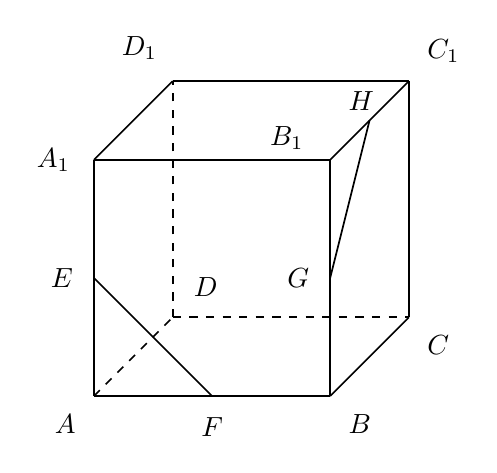
\begin{tikzpicture}[x=1cm,y=1cm,line width=0.6pt,font=\normalsize]
\coordinate (A) at (0,0);
\coordinate (B) at (3,0);
\coordinate (B1) at (3,3);
\coordinate (A1) at (0,3);
\coordinate (D) at (1,1);
\coordinate (C) at (4,1);
\coordinate (C1) at (4,4);
\coordinate (D1) at (1,4);
\coordinate (E) at (0,1.5);
\coordinate (F) at (1.5,0);
\coordinate (G) at (3,1.5);
\coordinate (H) at (3.5,3.5);
% front face solid
\draw (A) -- (B);
\draw (B) -- (B1);
\draw (B1) -- (A1);
\draw (A1) -- (A);
% top face solid
\draw (A1) -- (D1);
\draw (D1) -- (C1);
\draw (C1) -- (B1);
% right face solid
\draw (C1) -- (C);
\draw (B) -- (C);
% back/left dashed
\draw[dashed] (A) -- (D);
\draw[dashed] (D) -- (D1);
\draw[dashed] (D) -- (C);
% interior segments
\draw (E) -- (F);
\draw (G) -- (H);

% labels offset to avoid strokes
\node[below left,xshift=-3pt,yshift=-3pt] at (A) {$A$};
\node[below right,xshift=3pt,yshift=-3pt] at (B) {$B$};
\node[below right,xshift=3pt,yshift=-3pt] at (C) {$C$};
\node[above right,xshift=4pt,yshift=4pt] at (D) {$D$};
\node[left,xshift=-5pt,yshift=0pt] at (A1) {$A_{1}$};
\node[left,xshift=-6pt,yshift=8pt] at (B1) {$B_{1}$};
\node[above right,xshift=3pt,yshift=3pt] at (C1) {$C_{1}$};
\node[above left,xshift=-2pt,yshift=4pt] at (D1) {$D_{1}$};
\node[left,xshift=-4pt,yshift=0pt] at (E) {$E$};
\node[below,xshift=0pt,yshift=-4pt] at (F) {$F$};
\node[left,xshift=-4pt,yshift=0pt] at (G) {$G$};
\node[above,xshift=-3pt,yshift=0pt] at (H) {$H$};
\end{tikzpicture}
